\chapter{Ανάλυση αποτελεσμάτων}\label{ch:results}


\section{Υλοποίηση}\label{sec:implementation}
H υλοποίηση της μεθόδου k-Nearest Neighbor έγινε στη γλώσσα \texttt{C++} και πραγματοποιήθηκε
ως προσθήκη στην υπάρχουσα υλοποίηση της μεθόδου από τη βιβλιοθήκη \texttt{OpenCV} \flink{https://opencv.org}.
Για την μεταγλώττιση του κώδικα και την παραγωγή των εκτελέσιμων αρχείων χρησιμοποιήθηκε
ο μεταγλωττιστής \texttt{g++} με έκδοση \texttt{4:6.3.0-4} σε περιβάλλον \texttt{Debian Stretch Linux}.
Η πειραματική διάταξη υλοποιήθηκε στη γλώσσα \texttt{Python2.7} χρησιμοποιώντας
τους \texttt{python wrappers} της OpenCV. Όλα τα πειράματα εκτελέστηκαν σε υπολογιστή
\texttt{Intel(R) Core(TM) i7-2640M CPU @ 2.80GHz} χωρίς χρήση GPU. Για την αξιολόγηση
χρησιμοποιήθηκε το σύστημα της \texttt{k-fold Cross Validation}\flink{https://en.wikipedia.org/wiki/Cross-validation_(statistics)}.


\section{Πειραματική μεθοδολογία}\label{sec:methodology}
\subsection{Βάσεις δεδομένων}
Για τις μετρήσεις χρησιμοποιήθηκαν οι βάσεις δεδομένων προσώπων \texttt{AT\&T Facedatabase}
\flink{www.cl.cam.ac.uk/research/dtg/attarchive/facedatabase.html},
\texttt{Yale Facedatabase A}\flink{vision.ucsd.edu/content/yale-face-database},
\texttt{Extended Yale Facedatabase B}\flink{http://vision.ucsd.edu/~leekc/ExtYaleDatabase/ExtYaleB.html}
καθώς και μια βάση κατασκευασμένη από το συγγραφέα με βάση κάποιο πολυμεσικό πειραματικό
υλικό που δόθηκε από το Πανεπιστήμιο του Lucce\flink{https://www.imtlucca.it/}.

\begin{description}
  \item[AT\&T Facedatabase] \hfill \\
    Η βάση AT\&T Facedatabase περιέχει 10 διαφορετικές εικόνες για 40 διαφορετικά
    πρόσωπα. Για κάποια πρόσωπα οι εικόνες έχουν συλλεχθεί σε διάφορες χρονικές
    στιγμές, με ανομοιόμορφες συνθήκες φωτισμού και διαφορετικές εκφράσεις (χαμόγελο,
    ανοιχτά/κλειστά μάτια) και χαρακτηριστικά (πχ γυαλιά). Σε όλες τις εικόνες υπάρχει
    ομοιόμορφο μαύρο φόντο.
  \item[Yale Facedatabase A] \hfill \\
    Περιέχει 15 πρόσωπα και 11 ασπρόμαυρες φωτογραφίες για το καθένα από αυτά.
    Οι εικόνες έχουν μέγεθος $320x243$ pixel ενώ υπάρχουν διαφοροποιήσεις στις
    συνθήκες φωτισμού, στις εκφράσεις του προσώπου και τα χαρακτηριστικά. Στη
    βιβλιογραφία θεωρείτε πιο αξιόπιστη από την παραπάνω.\\
    \\
    Οι εικόνες των προσώπων των δύο αυτών βάσεων δεν είναι στις ακριβείς διαστάσεις
    των προσώπων και χρειάζονται μια προ-επεξεργασία για να μπορέσουν να αξιοποιηθούν.
  \item[Extended Yale Facedatabase B] \hfill \\
    Η βάση αυτή περιέχει 2414 εικόνες από 38 διαφορετικά πρόσωπα κομμένες ακριβώς
    στις διαστάσεις του κάθε προσώπου. Ο στόχος της βάσης είναι να μπορούν να εξαχθούν
    χαρακτηριστικά των προσώπων ανθεκτικά στις αλλαγές του φωτισμού. Για το λόγο αυτό
    όλα τα πρόσωπα έχουν σχεδόν τις ίδιες εκφράσεις και χαρακτηριστικά.
  \item[LucceFaces] \hfill \\
    Η βάση αυτή περιέχει 10 εικόνες για κάθε ένα από τα 12 πρόσωπα που περιέχει.
    Οι εικόνες των προσώπων εξήχθησαν από πραγματικό πολυμεσικό περιεχόμενο. Είναι
    μια βάση προσώπων για την αξιολόγηση του συγκεκριμένου dataset.
\end{description}

\subsection{Πρωτόκολλο αξιολόγησης}
Για την αξιολόγηση ενός αλγορίθμου αναγνώρισης προσώπων χρειάζεται να διαθέτουμε δύο
βάσεις δεδομένων εικόνων. Μια που να αποτελεί τη βάση με την οποία εκπαιδεύεται η
μέθοδος και μία πάνω στην οποία να εκτελείται. Το σχήμα που ακολουθήθηκε παρήγαγε
και τις δύο βάσεις από τις παραπάνω χρησιμοποιώντας την τεχνική Cross-validation\flink{https://en.wikipedia.org/wiki/Cross-validation_(statistics)}
Η μέθοδος εκτελείται $n$ επαναλήψεις  και σε κάθε μία αξιολογείται από τη μέθοδο
αξιολόγησης k-fold Cross-validation. Στο σύνολο των επαναλήψεων υπολογίζεται
η μέση ακρίβεια (accuracy). Η υλοποίηση της μεθόδου δίνει μία πρόβλεψη για κάθε
πρόσωπο η οποία είτε είναι σωστή (true positive) είτε λάθος (false positive).
Σε κάθε περίπτωση δεν έχουμε καθόλου true negatives και false negatives. Επομένως
στη συγκεκριμένη περίπτωση το μέτρο \textbf{\texttt{Accuracy}} που υπολογίζουμε ταυτίζεται με το \texttt{Precision}
ενώ το \texttt{Recall} θα παραμένει πάντα σταθερό και ίσο με 1. Το Precision και
το Recall είναι οι τυπικές μετρικές για την αξιολόγηση αλγορίθμο που πραγματοποιούν
ταξινόμηση κλάσης.

$$
Precision = \frac{tp}{tp + fp}
$$

$$
Recall = \frac{tp}{tp + fn}
$$


\paragraph{k-fold Cross Validation} \hspace*{3pt}\\
\\
Με τη μέθοδο αυτή χτίζονται k μη επικαλυπτόμενα σετ εκπαίδευσης και πειραματισμού
από την αρχική βάση δεδομένων. Έτσι αποφεύγονται συνθήκες όπου ολόκληρη η μέθοδος
είναι εκπαιδευμένη με χαρούμενα πρόσωπα ενώ το σετ εικόνων που χρησιμοποιείται στα
πειράματα περιέχει λυπημένα πρόσωπα. Παρακάτω παρουσιάζεται ένα μικρό παράδειγμα της
μεθόδου 4-fold Cross Validation:

\newpage


\begin{figure}[htbp]
  \begin{center}
    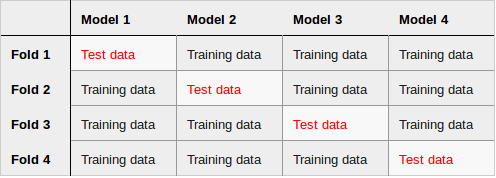
\includegraphics[width=0.8\maxwidth]{../figures/kfold.png}
    \caption{Η μέθοδος k-fold Cross Validation \label{fig:rcnn}}
   \end{center}
\end{figure}

Παρατηρούμε ότι σε κάθε επανάληψη (fold) επιλέγονται καινούργια και ανεξάρτητα
σετ εκπαίδευσης και πειραματισμού.

Η ακρίβεια που υπολογίζεται είναι ο μέσος όρος των τιμών της ακρίβειας που
υπολογίζονται σε κάθε fold.


\section{Αποτελέσματα}\label{sec:results}

Με βάση τα χαρακτηριστικά (αριθμός προσώπων και εικόνες) των βάσεων δεδομένων
που χρησιμοποιήσαμε επιλέξαμε να αξιολογήσουμε τη μέθοδο με \textbf{4-fold} και
\textbf{10-fold} cross validation για μεγαλύτερη αξιοπιστία στα αποτελέσματα.

Αξιολογήσαμε την τροποποιημένη μέθοδο για διαφορετικές τιμές του \textbf{k} και
για 3 διαφορετικά είδη αποστάσεων, την τυπική \textbf{Eucledian} απόσταση, την
\textbf{ChiSquare} και την \textbf{Cosine} απόσταση. Παρακάτω φαίνονται τα πειράματα
για τις 4 βάσεις δεδομένων.

Δίνονται οι ορισμοί των αποστάσεων:

\texttt{Ευκλείδεια απόσταση}
$$
d(H_1, H_2) = \sqrt{H_1^2 + H_1^2}
$$

\texttt{Chisquare απόσταση}
$$
d(H_1, H_2) = \sum{\frac{(H_1-H_2)^2}{H_1+H_2}}
$$

\texttt{Cosine απόσταση}
$$
d(H_1, H_2) = -\frac{H_1^T*H_2}{\sqrt{(H_1*H_1^T)x(H_2*H_2^T))}}
$$

\begin{figure}[htp]
    \centering
    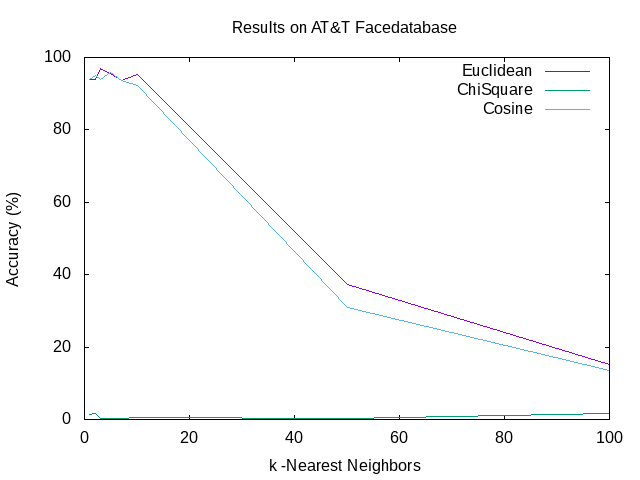
\includegraphics[width=.49\textwidth]{../figures/k4-att.pdf}\hfill
    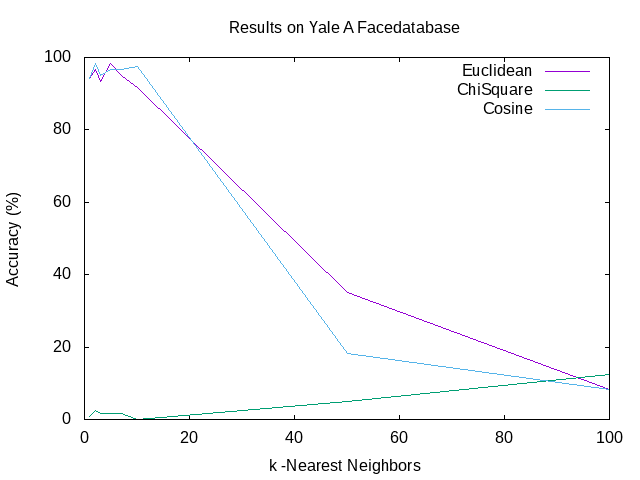
\includegraphics[width=.49\textwidth]{../figures/k4-yaleA.pdf}\hfill
    \includegraphics[width=.48\textwidth]{../figures/k4-yaleB.pdf}\hfill
    \includegraphics[width=.48\textwidth]{../figures/k4-lucce.pdf}\hfill

    \caption{k-4 cross validation}
    \label{fig:bee}

\end{figure}

\begin{figure}[htp]
    \centering
    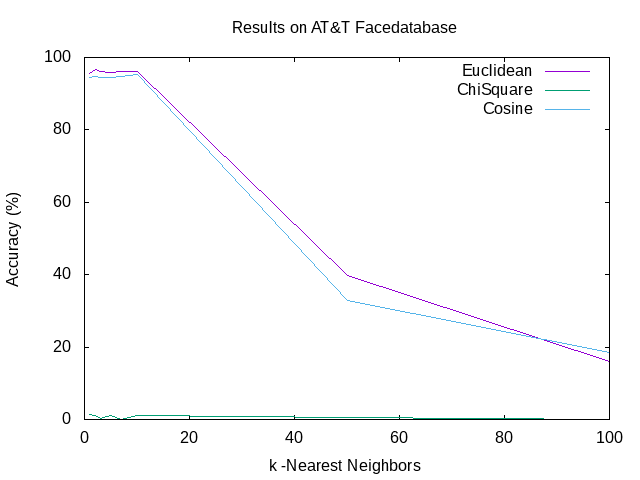
\includegraphics[width=.49\textwidth]{../figures/k10-att.pdf}\hfill
    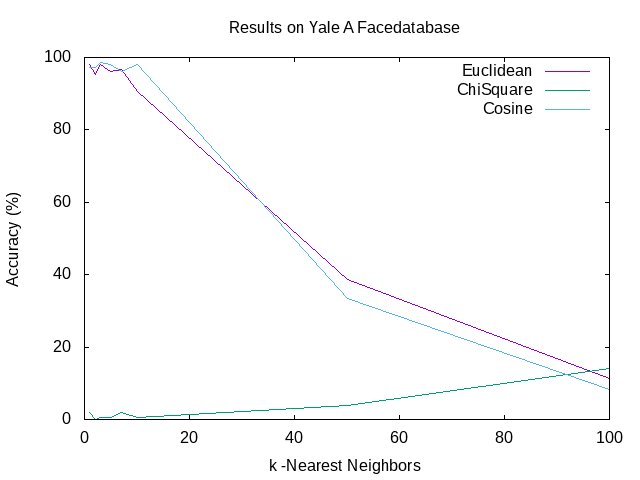
\includegraphics[width=.49\textwidth]{../figures/k10-yaleA.pdf}\hfill
    \includegraphics[width=.48\textwidth]{../figures/k10-yaleB.pdf}\hfill
    \includegraphics[width=.48\textwidth]{../figures/k10-lucce.pdf}\hfill

    \caption{k-10 cross validation}
    \label{fig:bee}

\end{figure}

Επίσης για διαφορετικές τιμές του \textbf{k} συγκρίναμε τη μέθοδό μας για την
τυπική Ευκλείδεια απόσταση και την Chisquare (που φαίνεται να υπερτερεί) με τη μέθοδο
\textbf{FisherFaces} ως τον εξαγωγέα των χαρακτηριστικών από το πρόσωπο.

\begin{figure}[htp]
    \centering
    \includegraphics[width=.49\textwidth]{../figures/k4-att-comp.pdf}\hfill
    \includegraphics[width=.49\textwidth]{../figures/k4-yaleA-comp.pdf}\hfill

    \caption{k-4 cross validation}
    \label{fig:bee}

\end{figure}

\begin{figure}[htp]
    \centering
    \includegraphics[width=.49\textwidth]{../figures/k10-att-comp.pdf}\hfill
    \includegraphics[width=.49\textwidth]{../figures/k10-yaleA-comp.pdf}\hfill

    \caption{k-10 cross validation}
    \label{fig:bee}

\end{figure}
